%
%  This simple example illustrates how documents can be
%  split into smaller segments, each segment processed
%  by latex2html separately.  This document can be
%  processed through latex and latex2html with the
%  corresponding makefile.
%

\documentclass{article}         % Must use LaTeX 2e
\usepackage[plainpages=false, colorlinks=true, citecolor=black, filecolor=black, linkcolor=black, urlcolor=black]{hyperref}		
\usepackage[left=.75in,right=.75in,top=.75in,bottom=.75in]{geometry}
\usepackage{makeidx,color,boxedminipage}
\usepackage{graphicx,float}
\usepackage{amsmath,amsthm,amsfonts,amscd,amssymb} 

%%%%%%%%%%%%%%%%%%%%%%%%%%%%%%%%%%%%%%%%%%%%%%%%%%%%%%%%%%%%%%%%%%%%%%
%	Some math support.					     %
%%%%%%%%%%%%%%%%%%%%%%%%%%%%%%%%%%%%%%%%%%%%%%%%%%%%%%%%%%%%%%%%%%%%%%
%
%	Theorem environments (these need the amsthm package)
%
%% \theoremstyle{plain} %% This is the default

\newtheorem{thm}{Theorem}[section]
\newtheorem{cor}[thm]{Corollary}
\newtheorem{lem}[thm]{Lemma}
\newtheorem{prop}[thm]{Proposition}
\newtheorem{ax}{Axiom}

\theoremstyle{definition}
\newtheorem{defn}{Definition}[section]

\theoremstyle{remark}
\newtheorem{rem}{Remark}[section]
\newtheorem*{notation}{Notation}
\newtheorem*{exrcs}{Exercise}
\newtheorem*{exmple}{Example}

%\numberwithin{equation}{section}


%%%%%%%%%%%%%%%%%%%%%%%%%%%%%%%%%%%%%%%%%%%%%%%%%%%%%%%%%%%%%%%%%%%%%%
%	Macros.							     %
%%%%%%%%%%%%%%%%%%%%%%%%%%%%%%%%%%%%%%%%%%%%%%%%%%%%%%%%%%%%%%%%%%%%%%
%
%	Here some macros that are needed in this document:

\newcommand{\motion}{\mathbf{\varphi}}
\newcommand{\hmotion}{\mbox{\boldmath $\hat{\varphi}$}}
\newcommand{\cauchy}{\mbox{\boldmath $\sigma$}}
\newcommand{\eqn}[1]{(\ref{#1})}
\newcommand{\hOmega}{\hat{\Omega}}
\newcommand{\homega}{\hat{\omega}}
\newcommand{\nphalf}{n+\frac{1}{2}}
\newcommand{\nmhalf}{n-\frac{1}{2}}
\newcommand{\kmhalf}{k-\frac{1}{2}}
\newcommand{\kphalf}{k+\frac{1}{2}}
\newcommand{\picdir}{pdffig/}

\newcommand{\re}{\mathbb R}
\newcommand{\Ex}[2]{\mathcal{E}^{#2}[#1]}
%\newcommand{\log}{\text{log}[#1]}
\newcommand{\Tr}{\mathbf{Tr}}
\newcommand{\etal}{\textit{et al. }}

\newcommand{\eq}[1]{Eq.~(\ref{#1})}
\newcommand{\Fig}[1]{Fig.~\ref{#1}}

\renewcommand{\v}[1]{\ensuremath{\mathbf{#1}}}
\newcommand{\vo}[1]{\ensuremath{\boldsymbol{#1}}}
\newcommand{\pderiv}[2]{\frac{\partial #1}{\partial #2}}

\newcommand{\eps}{\boldsymbol{\epsilon}}
\newcommand{\Nu}{\boldsymbol{\nu}}
\newcommand{\Ps}{\boldsymbol{\Psi}}
\newcommand{\xii}{\boldsymbol{\xi}}
\newcommand{\Al}{\boldsymbol{\alpha}}
\newcommand{\x}{\mathbf{x}}
\newcommand{\s}{\mathbf{s}}
\newcommand{\C}{\mathbf{C}}
\newcommand{\uu}{\mathbf{u}}
\newcommand{\z}{\mathbf{z}}
\newcommand{\q}{\mathbf{q}}
\newcommand{\A}{\mathbf{A}}
\newcommand{\B}{\mathbf{B}}
\newcommand{\K}{\mathbf{K}}
\newcommand{\f}{\mathbf{f}}
\newcommand{\hc}{\mathbf{H}}
\newcommand{\R}{\mathbf{R}}
\newcommand{\G}{\mathbf{G}}
\newcommand{\y}{\mathbf{y}}
\newcommand{\Y}{\mathbf{Y}}
\newcommand{\teta}{\boldsymbol{\theta}}
\newcommand{\Teta}{\boldsymbol{\Theta}}
\newcommand{\pe}{\hat{\mathbf{p}}}
\newcommand{\pl}{\mathbf{p}^{(l)}}
\newcommand{\pt}{\mathbf{p}^\text{true}}

\newcommand{\kk}{\mathcal{K}}
\newcommand{\p}{\mathcal{P}}
%\DeclareMathOperator{\Exp}{E}
\newcommand{\V}{{\mathpzc{V}}}
\newcommand{\E}{{\mathpzc{E}}}

\newcommand{\bs}{b}
\newcommand{\bv}{\mathbf{b}}
\newcommand{\bme}{z}
\newcommand{\bvm}{\tilde{\bv}}
\newcommand{\xg}{x^G}
\newcommand{\yg}{y^G}
\newcommand{\kbf}{\mathbf{k}}
\newcommand{\mbf}{\mathbf{m}}
\newcommand{\Pbf}{\mathbf{P}}
\newcommand{\Rbf}{\mathbf{R}}
\newcommand{\Vbf}{\mathbf{V}}
\newcommand{\xbf}{\mathbf{x}}
\newcommand{\Xbf}{\mathbf{X}}
\newcommand{\Ybf}{\mathbf{Y}}
\newcommand{\zbf}{\mathbf{z}}
\newcommand{\Zbf}{\mathbf{Z}}
\newcommand{\mubf}{\boldsymbol{\mu}}
\newcommand{\nubf}{\boldsymbol{\nu}}
\newcommand{\im}{\mathrm{i}}
\newcommand{\Gammabf}{\mathbf{\Gamma}}
\newcommand{\Cbf}{\mathbf{C}}
\newcommand{\Sigmabf}{\boldsymbol{\Sigma}}
\newcommand{\zcond}{\mathbf{z}\mid\mu}
\newcommand{\zcondbf}{\mathbf{z}\mid\boldsymbol{\mu}}
\newcommand{\signalG}{\mathcal{G}\paren{\mu,\mathbf{k}}}
\newcommand{\Gscript}{\mathcal{G}}
\newcommand{\sumnn}{\sum\limits_{n=1}^N}

\newcommand{\arr}[2]{\begin{array}{#1} #2 \end{array}}
\newcommand{\lbrcarray}[2]{\left\{\arr{#1}{#2}\right.}
\newcommand{\rbrcarray}[2]{\left.\arr{#1}{#2}\right\}}
\newcommand{\argminx}{\arg\min_X}
\newcommand{\Nscript}{\mathcal{N}}

%\DeclareMathOperator{\diag}{diag} 
\newcommand{\brkarray}[2]{\bracket{\arr{#1}{#2}}}

\title{Advanced Applications of Synthetic MR and MAGiC}
\author{}
\begin{document}                % The start of the document
\maketitle

%%%%%%%%%%%%%%%%%%%%%%%%%%%%%%%%%%%%%%%%%%%%%%%%%%%%%%%%%%%%%%%%
\section{Paper Outline Tasks}
%%%%%%%%%%%%%%%%%%%%%%%%%%%%%%%%%%%%%%%%%%%%%%%%%%%%%%%%%%%%%%%%
\begin{itemize}
\item @fuentesdt Code Eq. \eqn{mimax}
\item @fuentesdt generate MI map of high information content regions, Figure~\ref{fig:MIMapTDTE}
\item {\color{red} @kenphwang Need 2 data sets. (1) phantom with known T1/T2 and (2) example data set  in human. is this real/imaginary data? }
\item {\color{red} Recon all data sets with current $TE$ and $TD$ and optimal $TE$ and $TD$.  @kenphwang can we get the current code for this recon? }
\item @fuentesdt compare and report accuracy in the optimal vs current recon technique
\end{itemize}

%%%%%%%%%%%%%%%%%%%%%%%%%%%%%%%%%%%%%%%%%%%%%%%%%%%%%%%%%%%%%%%%
%%%%%%%%%%%%%%%%%%%%%%%%%%%%%%%%%%%%%%%%%%%%%%%%%%%%%%%%%%%%%%%%
\section{Problem Statement}\label{sec:prob_statement}
%%%%%%%%%%%%%%%%%%%%%%%%%%%%%%%%%%%%%%%%%%%%%%%%%%%%%%%%%%%%%%%%
%%%%%%%%%%%%%%%%%%%%%%%%%%%%%%%%%%%%%%%%%%%%%%%%%%%%%%%%%%%%%%%%
Consider a \textbf{complex} magnetization signal $M_{TD} \in \mathbb{C}$ that
is defined as as function of \textbf{acquisition parameters} 
$\kk=\{\vec{k},T_R,T_D,\theta,T_E,\alpha\}$ 
and \textbf{tissue properties} $\p \equiv \{T_1,T_2,M_0\}$. 
Within the scope of this project, $T_R$=4sec, $\theta$=120\textsuperscript{o}, 
and $\alpha$=90\textsuperscript{o} are \textbf{fixed}. Delay time, $T_D$, echo time $T_E$,
and $k-$space location, $\vec{k}$, are parameters under consideration for
acquisition optimization. 


\begin{figure}[h] 
\centering
\begin{tabular}{ccc}
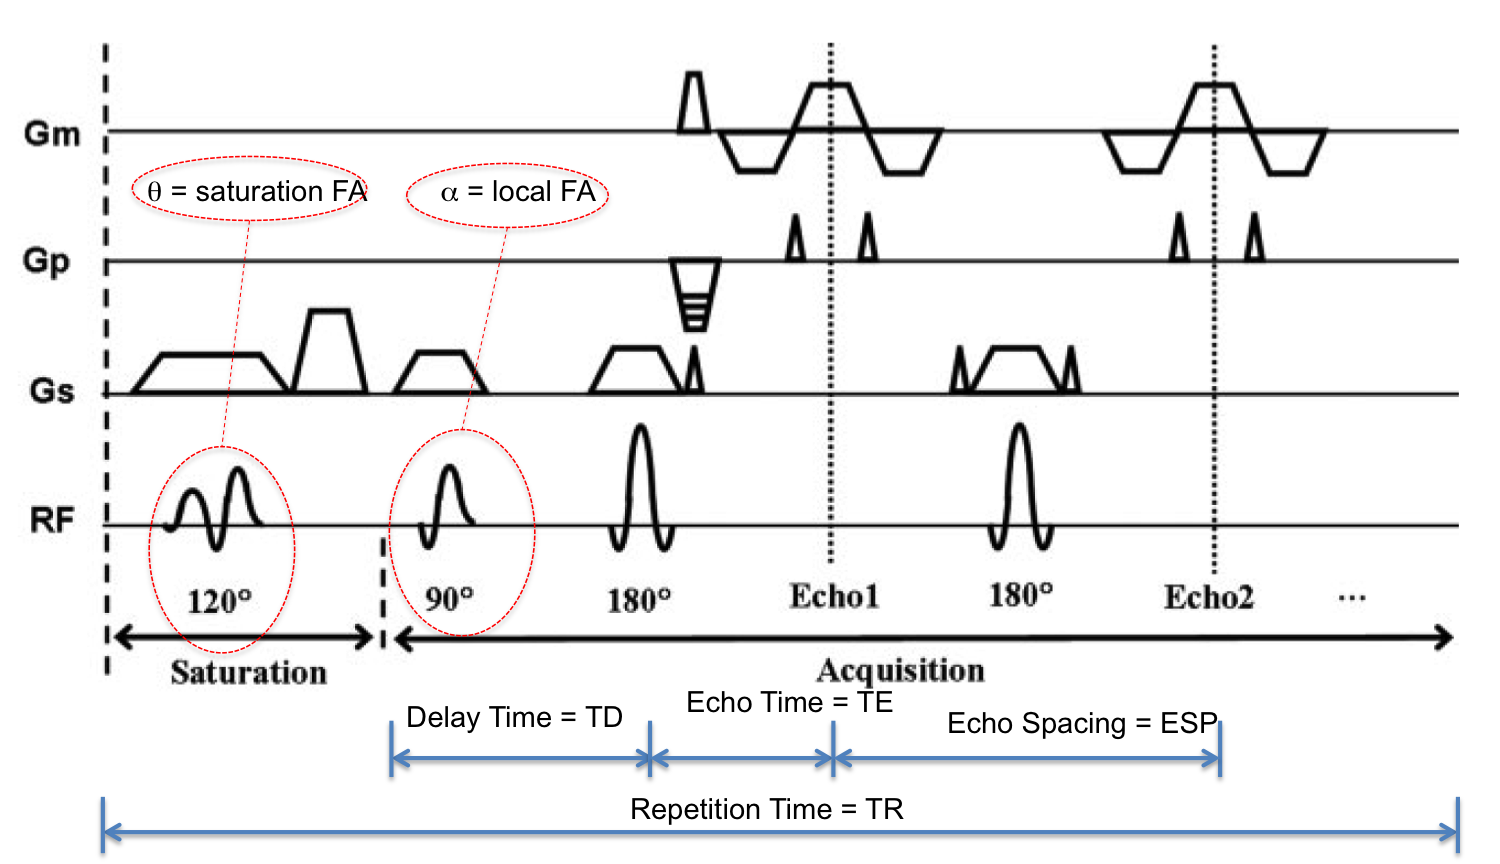
\includegraphics[width=.7\textwidth]{\picdir/PulseSequence.png} & 
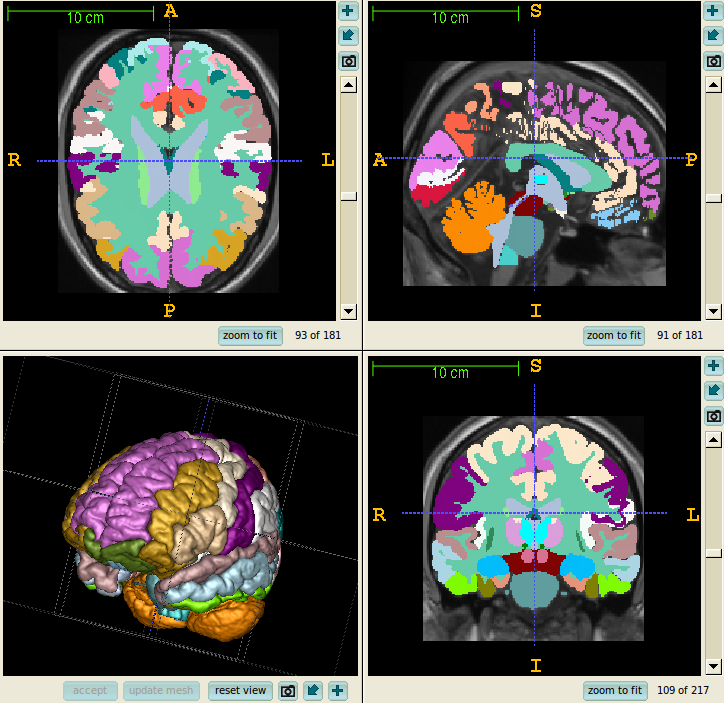
\includegraphics[width=.29\textwidth]{\picdir/NeuroBasis.png} \\
(a) & (b) \\
\end{tabular}
\caption{ 
(a) Synthetic MR Pulse sequence. (b) Neuroimaging basis.
}\label{fig:Pulsesequence}
\end{figure}

\begin{equation}\label{mtd}
M_{TD}(T_R,T_D,\theta,T_E,\alpha,\p,\x)=
   M_0(\x) e^{i\psi(\x)}
\left(
 \frac{1-(1-\cos \theta)e^{-\frac{T_D}{T_1(\x)}}-\cos \theta e^{-\frac{T_D}{T_1(\x)}}}{1-\cos \theta e^{-\frac{T_R}{T_1(\x)}}cos \alpha}
 \right) e^{-\frac{T_E}{T_2(\x)}}
\end{equation}
Here, $M_0$ is the unsaturated magnetization, $\psi(\x)$ is the measured phase offset,
$\theta$ represents the \textit{saturation} flip
angle, and $T_R$ and $T_E$ denote repetition time and echo time, respectively.
Parameters $T_1$ and $T_2$ represents relaxation times, and $\alpha$ is the
\textit{local} excitation flip angle. 
In general, excitation pulse $\alpha$ is a function of flip angle, i.e.
$\alpha=\alpha(\theta)$
{\color{red}(@kenphwang why is this?)}.
Note that the unsaturated magnetization $M_0$, along with
relaxation times $T_1$ and $T_2$, are a function of spatial coordination $\x$.
Basis functions $\phi_i$ represent the neuroanatomy. For completeness, consider
$\phi_1 = \phi_\text{gm}$,
$\phi_2 = \phi_\text{wm}$,
$\phi_3 = \phi_\text{csf}$,
$\phi_4 = \phi_\text{tumor}$ as a simplified set 
of the regions illustrated in Figure~\ref{fig:Pulsesequence}(b).
\[
T_1(\xbf)=\sum_{i=1}^{N=4} T1_i \phi_i(\xbf)
\qquad
T_2(\xbf)=\sum_{i=1}^{N=4} T2_i \phi_i(\xbf)
\qquad
M_0(\xbf)=\sum_{i=1}^{N=4} M0_i \phi_i(\xbf)
\]
	
	
\[
\bigcup_{i=1}^{N=4}\Omega_i=\Omega  \qquad  \Omega_n\cap\Omega_m=\varnothing
\qquad 
\phi_i(\xbf)=\left\{ \begin{split}
			1 & \quad x\in\Omega_i \\
			0 & \quad \text{otherwise}
                     \end{split} \right. 
\]

Under the assumptions:
\begin{itemize} 
 \item phase offset, $\psi(\x)$, constant over acquisition time 
 \item TE = effective echo time when readout crosses $k-$space center, i.e.  ignore additional
       T2$^*$ decay of echo train
 \item constant gradients 
        \[ \left\{
             \begin{split}
           k_x & = \gamma G (t - TE) \\
           k_y & = \gamma  G_y T_{pe} \\
           k_z & = \gamma  G_z T_{pe} \\
           \end{split}
           \right. \qquad
          |t-TE| < T_{acq}/2
          \qquad \qquad
          \vec{k} \equiv \frac{\gamma \; \vec{G} \; t}{2 \pi}
        \]
The time in this signal model, $t$, represents the measurements during
the readout and is less the the repetition time $t < TR \approx 500ms$.
\[
  t =  iii \cdot \Delta t \quad iii = 0, ..., 255
\qquad 
  \Delta t = \frac{T_{acq}}{256} 
\]
Note that the acquisition time for a single echo/single slice under this model may be
estimated as the number of phase encodes times the repetition time.
\[
   \text{acquisition time} = \# \text{phase encodes } \cdot TR 
                           \leq 256 \cdot 500ms \approx 2 \text{min}
\]

\end{itemize} 

The $k-$space measurements, $\mathcal{G} \in \mathbb{C}$, have the intuitive interpretation
as the Fourier coefficients of the complex image weight by the
coil sensitivities, $c(r):  \mathbb{R}^3 \rightarrow \mathbb{R}$.
 
\begin{equation}
\label{FFTmultiecho}
\begin{split}
\mathcal{G}(k_x,k_y,k_z,T_R,T_D,\theta,T_E,\alpha,\p) 
  & = \text{Fourier transform} \left\{ \underbrace{c_l(r) M_{TD}(T_R,T_D,\theta,T_E,\alpha,\p,r) }_{\equiv f(r):\mathbb{R}^3 \rightarrow \mathbb{C} } \right\}
          = \mathcal{F}(f(r))
\\
 & = \int_\Omega \left(M_{TD}(T_R,T_D,\theta,T_E,\alpha,\p,r)c_l(r)  \right)
          e^{-2  \pi i \vec{k}  \cdot r } \; dr
\end{split}
\end{equation}

Assuming the real and imaginary components of the signal are independent Gaussian noise our 
signal model may equivalently be understood in $\mathbb{R}^2$ in terms of the real
and imaginary components.
\[
\begin{bmatrix}
z_r(k_x,k_y,k_z,T_R,T_D,\theta,T_E,\alpha,\p) \\
z_i(k_x,k_y,k_z,T_R,T_D,\theta,T_E,\alpha,\p) \\
\end{bmatrix}
= 
\begin{bmatrix}
\Re \left\{ \mathcal{G}(k_x,k_y,k_z,T_R,T_D,\theta,T_E,\alpha,\p)  \right\} \\
\Im \left\{ \mathcal{G}(k_x,k_y,k_z,T_R,T_D,\theta,T_E,\alpha,\p)  \right\} \\
\end{bmatrix}
 + 
\begin{bmatrix}
\nu_r \\
\nu_i \\
\end{bmatrix}
\]
For similicity in notation, vector notation will be assumed.
\[\boxed{
z(\kk,\p) = \mathcal{G}(\kk,\p) + \nu
\qquad
\nu \sim N(0,\R)
\qquad
\R = 
\begin{bmatrix}
\sigma_z &      0    \\
    0    & \sigma_z  \\
\end{bmatrix}
\quad
\sigma_z \in \mathbb{R}
}
\]

Note that the observation $z$ is a function of control parameters $\kk$ and
parameters of interest $\p$.  The ultimate goal is to provide accurate estimate
of the parameters $\p$, given some measurements $z$. 
Precise estimation of parameters $\p$ crucially depends on the values of
control parameters $\kk=\{\vec{k},T_D,T_E\}$ ( $\{T_R,\theta,\alpha\}$ \textbf{fixed}).  
In other words, to ensure
performance of the estimation algorithm, one needs to select the control
parameters $\kk=\{\vec{k},T_D,T_E\}$ such that the observation $z$ provides
useful information about the parameters $\p$. This is achieved my maximizing
the mutual information between the measurements $z$ and parameters of interest
$\p$. 


\subsection{Alternative Image Space Formulation}
Assume that the signal model  for $M_{TD}$ \eqn{mtd} is our measurment model in \textbf{image space}
and is polluted with a white noise $\nu$ (with mean zero and variance $\R$). Hence, \eq{mtd} can be written as:
\begin{equation}\label{mtdobs}
z(\kk,\p)=\underbrace{M_{TD}(\kk,\p,\x)}_{\mathcal{G}(\kk,\p)}+\nu
\qquad
\nu \in \mathbb{R}^2
\quad 
\R = 
\begin{bmatrix}
\sigma_r &      0    \\
    0    & \sigma_i  \\
\end{bmatrix}
\end{equation}



%%%%%%%%%%%%%%%%%%%%%%%%%%%%%%%%%%%%%%%%%%%%%%%%%%%%%%%%%%%%%%%%
\section{ Mathematical Framework}\label{GeneralMathFramework}
%%%%%%%%%%%%%%%%%%%%%%%%%%%%%%%%%%%%%%%%%%%%%%%%%%%%%%%%%%%%%%%%

The underlying philosophy and assumptions within our approach is that the physics 
models are 1st order accurate or within 70-80\% of the needed accuracy and the error is
adequate within the assumed Gaussian noise.
Gaussian distributions provide analytical representations of the random
variables of interest (ie T1, T2) within the Bayesian setting and 
provide a crux for understanding. In particular, we say that a random
variable $\eta$ belongs to a multi-variate normal distribution 
of mean $\mu \in \mathbb{R}^n $ and covariance $\Sigma \in \mathbb{R}^{n \times n}$
\[
     \eta \sim \mathcal{N}(\mu,\Sigma)  
    \Rightarrow
      p(\eta)  = \frac{1}{2 \; \pi \; \det{\Sigma}} \exp\left( - \frac{1}{2} \| \mu - \eta\|^2_{\Sigma}\right)
\]


\begin{enumerate}
  \item Our data acquistion model, $\mathcal{G}(\kk,\p): \mathbb{R}^a
\times \mathbb{R}^m \rightarrow \mathbb{R}^n $,
maps deterministic acquisition
parameters, $\kk \in \mathbb{R}^a$, and uncertain parameters, $\p \in \mathbb{R}^m$
to observables, $\vec{z} \in \mathbb{R}^n$ ( or $\vec{z} \in \mathbb{C}^n$).
Explicitly, we will assume that the
measurement models are corrupted by zero mean white noise noise of a
\textbf{known} covariance matrix, $\Sigma_z \in \mathbb{R}^{n \times n}$ 
\begin{equation}
\label{sensormodelstructure}
\begin{split}
  \vec{z} & = \mathcal{G}(\kk;\p) + \nu   \qquad   \nu \sim \mathcal{N}(0,\Sigma_z)
     \end{split}
\end{equation}
$\nu$ may be interpreted as the measurement noise or the acquisition noise
in the sensor model. For a deterministic measurement model $\mathcal{G}$,
the conditional probablity distribution has an explicit analytical form
and may be written as a  \textbf{known} Gaussian
distribution. 
  \[ 
      p(z|\p)   =  \mathcal{N}(\mathcal{G}(\kk;\p),\Sigma_z)  
                      =  \frac{1}{2 \; \pi \; \det{\Sigma_z}} \exp\left( - \frac{1}{2} \|\mathcal{G}(\kk;\p)  - z \|^2_{\Sigma_z}\right)
  \]
  \item Additional \textbf{known} information is the prior probability
distributions for the model parameters, $p(\p)$.  For simplicity,
    assume that Prior parameters are Gaussian distributed of 
   \textbf{known} mean, $\hat{\p}$ and covariance, $\Sigma_\p$
   \[
      \p \sim \mathcal{N} (\hat{\p}, \Sigma_\p)
                      =  \frac{1}{2 \; \pi \; \det{\Sigma_\p}} \exp\left( 
          - \frac{1}{2} \|\hat{\p}  - \p \|^2_{\Sigma_\p}
                                                                  \right)
   \]
We will consider the tissue properties to be
normally distributed Gaussian parameters.
\[
  \text{T1}_\text{WM}    =  \mathcal{N}(100ms, 20ms)  \qquad
  \text{T1}_\text{GM}    =  \mathcal{N}(120ms, 20ms)  \qquad
  \text{T1}_\text{CSF}   =  \mathcal{N}(320ms, 20ms)  \qquad
  \text{T1}_\text{Tumor} =  \mathcal{N}(300ms, 20ms)
\]
\[
  \text{T2}_\text{WM}    =  \mathcal{N}(100ms, 20ms)  \qquad
  \text{T2}_\text{GM}    =  \mathcal{N}(120ms, 20ms)  \qquad
  \text{T2}_\text{CSF}   =  \mathcal{N}(320ms, 20ms)  \qquad
  \text{T2}_\text{Tumor} =  \mathcal{N}(300ms, 20ms)
\]
\[
  \text{M0}_\text{WM}    =  \mathcal{N}(100??, 20??)  \qquad
  \text{M0}_\text{GM}    =  \mathcal{N}(120??, 20??)  \qquad
  \text{M0}_\text{CSF}   =  \mathcal{N}(320??, 20??)  \qquad
  \text{M0}_\text{Tumor} =  \mathcal{N}(300??, 20??)
\]
{\color{red}(@kenphwang need exact numbers)}

  \item Bayes theorem is fundamental to the approach, Appendix~\ref{IntuitiveBayes}.
The probability of the measurements $p(z)$ must be interprited in terms of the
known information. The probability of the measurements may be derived from
the marginalization of the joint probability and has the interpretation as
the projection of the joint probability onto the measurement axis.
\[ 
\begin{split}
p(z) & = \int_\p p(\p,z)  \; d\p  
       = \underbrace{
         \int_\p 
          p(z|\p) \; p(\p)\; d\p  
          }_{
         \int_\p  =
              \int_{\text{T1}_\text{WM}     }
              \int_{\text{T1}_\text{GM}     }
              \int_{\text{T1}_\text{CSF}    }
              \int_{\text{T1}_\text{Tumor}  }
              \int_{\text{T2}_\text{WM}     }
              \int_{\text{T2}_\text{GM}     }
              \int_{\text{T2}_\text{CSF}    }
              \int_{\text{T2}_\text{Tumor}  }
              \int_{\text{M0}_\text{WM}     }
              \int_{\text{M0}_\text{GM}     }
              \int_{\text{M0}_\text{CSF}    }
              \int_{\text{M0}_\text{Tumor}  }
            }
    \\
     & = C 
          \int_\p
            \; d\p  
               \exp\left( - \frac{1}{2} \left(
                     \|\mathcal{G}(\kk;\p)  - z \|^2_{\Sigma_z}
                   + \|\hat{\p}  - \p \|^2_{\Sigma_\p}
                  \right)              \right)
       = C 
          \int_\p
            \; d\p  
               \exp\left( - \frac{1}{2} \left(
                     \|\mathcal{F}M_{TD}  - z \|^2_{\Sigma_z}
                   + \|\hat{\p}  - \p \|^2_{\Sigma_\p}
                  \right)              \right)
\end{split}
\]
  \item  The concept of informational entropy~\cite{madankan2015accelerated}, $H(Z)$,
provides a mathematically rigorous framework to look for measurement acquisition
parameters, $\kk$, with the high information content of the reconstruction, Figure~\ref{Fig:entropy}.
Given a probability space 
$(\Omega, \mathcal{F},p)$ (probability maps from the
sigma-algebra of possible events $p:\mathcal{F}\rightarrow [0,1]$
sigma-algebra, $\mathcal{F}$, defined on set of `outcomes' $\Omega$
\cite{durrett2010probability}),
we will define information of an event  as
proportional to the inverse probability.
\[
\text{information} \equiv  \frac{1}{p(z)}
\]
Intuitively, when a low probability event occurs this provides high
information.
The informational entropy is an \textit{average}
of the information content for a sigma algebra of events $\mathcal{F}$
\[
H(Z) = \int_Z  p(z) \ln\frac{1}{p(z)} \; dz
\qquad
  p(z) = \int_\p p(z|\p) \; p(\p)\; d\p 
\]
Hence this entropy measure is an average of the information content
for a given set of events, $\mathcal{F}$, and is proportional to the
variance or uncertainty in which the set of events occur.
This agrees with thermodynamic entropy;
if the information containing events are completely spread out such as in a
uniform distribution, the entropy is maxmized.
The entropy
is zero for a probability distribution in which
only one event occurs. Zero information is gained when the same event
always occurs ($0 \ln\frac{1}{0} = 0$). 

\begin{figure}[h]
Given a discrete probability function 
\[
p: \Omega \rightarrow \mathbb{R}^+
\qquad
  \Omega \equiv
\left\{
\begin{split}
c_i
= 
[a+i \; dx , a + (i+1) dx ) & \subset [a,b]
\\
& i = 0,..., N =   (b-a)/dx -1
\end{split}
\right\}
\qquad
 \sum_{i=1}^N  \underbrace{p(c_i)}_{ \equiv p_i} = 1
\]
\begin{minipage}{.7\textwidth}
Recall $\log \frac{x}{y} = \log x - \log y$,
       $\log x\; y       = \log x + \log y$.
The entropy is defined as:
\[
H(p)=-\sum_i p_i \log(p_i)
    =+\sum_i p_i ( \underbrace{\log 1}_{0} -  \log(p_i) ) 
    = \sum_i p_i \log\left(1/p_i\right)
\]
\end{minipage}~\begin{minipage}{.29\textwidth}
\scalebox{0.31}{\includegraphics*{\picdir/ProbInformation.png}} 
\end{minipage}

Here we are using a frequentist interpretation of probability.
I.e. $p_0 = 1 \Rightarrow$  the event occurs 10 out of 100 times.
\centering
\begin{tabular}{cc}
\scalebox{0.41}{\includegraphics*{\picdir/EntropyBins.png}} 
&
\scalebox{0.41}{\includegraphics*{\picdir/EntropyValue.png}} 
\end{tabular}
\caption{Entropy.
Similar to thermodynamics, the entropy
is a measure of the spread or uncertainty in a probability
distribution. A uniform probability distribution has the largest entropy.
This agrees within our intuition. If we have relatively little information
about a model parameter/variable, then it can be anywhere uniformly within
the interval. The more information we have the more `peaked' the probability
distribution. For example, suppose  an object is located with uniform
probability, $x \sim \mathcal{U}[a,b]$. The object is located 
between $[a,b]$ with equal probability and we are uncertain were it may
actually be. Compared to $x \sim \mathcal{N}[(a+b)/2,1]$, we are more
certain that the object is likely to be located near the mid-point
so we have relatively more information about the location of the object.
}\label{Fig:entropy}
\end{figure}
\item
Performance of estimation process crucially depends on the
value of control parameters $\kk$. Hence, it is important to develop
mathematical tools to identify the control parameters $\kk$ such that they
provide the best observation data for accurate estimation of parameter $\p$.
This is equivalent with maximizing the mutual information between the
observation data and parameters $\p$. Based on information theory, mutual
information is defined as the reduction of uncertainty in one parameter due to
knowledge of the other parameter.

\begin{equation} \label{mi}
I(\p;z)=\int_z\int_p p(\p,z)\ln\left(\frac{p(\p,z)}{p(\p)p(z)}\right)d\p dz
\end{equation}

We make use of Bayes theorem to simplify the above equation. By substituting $p(\p,z)$ with $p(z|\p)p(\p)$, \eq{mi} can be written as:

\begin{equation} \label{mi2}
I(\p;z)=\int_z\int_p p(z|\p)p(\p)\ln\left(\frac{p(z|\p)p(\p)}{p(\p)p(z)}\right)d\p dz
\end{equation}
Or,
\begin{equation} \label{mi3}
I(\p;z)=\int_z\int_p p(z|\p)p(\p)\ln\left[p(z|\p)\right]d\p dz - \int_z p(z) \ln p(z)dz
= H(Z) - H(Z|\p)
\end{equation}


Note that due to dependence of observation data $z$ on control parameters, the
mutual information $I(\p;z)$ is a function of control parameter $\kk$. In order
to maximize the reduction of uncertainty in parameter estimate (i.e. to have
the most confident estimates of the parameter $\p$), one can simply maximize
the mutual information between the observation data and parameters of interest:

\begin{equation}\label{mimax}
\max_{\kk \in \mathcal{F}} I(\p;z)
\qquad
\kk=\{\vec{k},T_D,T_E\} \in \mathcal{F} = 
   [\vec{k}_\text{lb},\vec{k}_\text{ub}] \times 
   (0,4sec] \times (0,140ms] \subset  \mathbb{Z}^3 \times \mathbb{R}^2 
\end{equation}
\end{enumerate}


%%%%%%%%%%%%%%%%%%%%%%%%%%%%%%%%%%%%%%%%%%%%%%%%%%%%%%%%%%%%%%%%
\subsection{Mutual Information Approximation}
%%%%%%%%%%%%%%%%%%%%%%%%%%%%%%%%%%%%%%%%%%%%%%%%%%%%%%%%%%%%%%%%
{\color{red} @dmitchell412 need entropy approximations here}

By assumption of Gaussian noise, $H(Z|\p)$ is constant.
Maximizing mutual information reduces to maximizing the entropy 
in the measurements.
Intuitively, we want to find acquisition parameters,
$\kk$, for which the measurements are most uncertain
Probilistic integrals may be computed from uncertainty quantification
techniques using kernel density methods (KDM) about quadrature 
points~\cite{walters2009estimation,
tobin2013kernel,terejanu2012bayesian,fahrenholtz2013generalised}.
\[
\max_\kk I(\p;z)
\propto
\max_\kk H(Z)
  \quad \Leftrightarrow \quad
\max_\kk 
    \int_Z   dz \underbrace{\int_\p  d\p \; p(z|\p) \; p(\p)}_{p(z)}
                \underbrace{ln \left(\int_\p  d\p \; p(z|\p) \; p(\p)\right)}_{ln \; p(z)}
\]
\[
    p(z) = 
         C \int_\p
            \; d\p  
              \exp\left( - \frac{1}{2} \left(
                     \|\mathcal{F}M_{TD}  - z \|^2_{\Sigma_z}
                   + \|\hat{\p}  - \p \|^2_{\Sigma_\p}
                  \right)              \right)
\]

To build intuition, Jensen inequality suggests that the expected value
may be used to bound the entropy from below.
\[
ln \; ( E[Z] ) \leq
E[ln\; p(z)] = H(z)  
\]

\[
 E[Z] = \int_Z   dz \; p(z) 
      = \int_Z   dz  \;
         C \int_\p
            \; d\p  
              \exp\left( - \frac{1}{2} \left(
                     \|\mathcal{F}M_{TD}  - z \|^2_{\Sigma_z}
                   + \|\hat{\p}  - \p \|^2_{\Sigma_\p}
                  \right)              \right)
\]

Further, \cite{madankan2015accelerated} showed that the variance is a reasonable
approximation to the entropy. Quadrature rules may be used to build
intuition on expect maximal locations.
\[
 H(z)   \propto H(\mathcal{F}M_{TD} )
   \approx E\left[\mathcal{F}M_{TD} - \mu\right]^2
   \approx \sum_{p=1}^Q \omega_p \left( \mathcal{F}M_{TD}(\p_p) \right)^2
\]
Resulting in 
\[
   \max_{\vec{k},TE,TD} \sum_{p=1}^Q \omega_p \left(
     \int_\Omega M_{TD}(T_D,T_E,\p_p,r)
          e^{-2  \pi i \vec{k}  \cdot r } \; dr
     \right)^2
\]

%%%%%%%%%%%%%%%%%%%%%%%%%%%%%%%%%%%%%%%%%%%%%%%%%%%%%%%%%%%%%%%%
%%%%%%%%%%%%%%%%%%%%%%%%%%%%%%%%%%%%%%%%%%%%%%%%%%%%%%%%%%%%%%%%
\subsection{Analytic Geometry}
%%%%%%%%%%%%%%%%%%%%%%%%%%%%%%%%%%%%%%%%%%%%%%%%%%%%%%%%%%%%%%%%
%%%%%%%%%%%%%%%%%%%%%%%%%%%%%%%%%%%%%%%%%%%%%%%%%%%%%%%%%%%%%%%%

Suppose for example that the magnetization function was of the form of a complex Gaussian.
\[
   M_{TD} = T1 \left( e^{i \pi x^2}
                    + e^{i \pi y^2}
                    + e^{i \pi z^2}
               \right)
  \qquad
  \Rightarrow
  \qquad
  \mathcal{F} M_{TD} =
            T1 \left(  e^{i \pi (1/4 - k_x^2)}
                     + e^{i \pi (1/4 - k_y^2)}
                     + e^{i \pi (1/4 - k_z^2)}
               \right)
\]
For a simple 1D geometry
\[
    p(z) = 
         C \int_{T1}
            \; dT1 \;   
              \exp\left( - \frac{1}{2} \left(
                     \|T1 \; e^{i \pi (1/4 - k_x^2)}  - z \|^2_{\Sigma_z}
                   + \|\hat{T1}  - T1 \|^2_{\Sigma_\p}
                  \right)              \right)
\]
{\color{red} @dmitchell412 need regression test.  What analytic form of
$M_{TD}$ should be assumed such that this integral is analytic ?  }

%%%%%%%%%%%%%%%%%%%%%%%%%%%%%%%%%%%%%%%%%%%%%%%%%%%%%%%%%%%%%%%%
%%%%%%%%%%%%%%%%%%%%%%%%%%%%%%%%%%%%%%%%%%%%%%%%%%%%%%%%%%%%%%%%
\section{Optimal ($T_D$,$T_E$) Design}\label{oed}
%%%%%%%%%%%%%%%%%%%%%%%%%%%%%%%%%%%%%%%%%%%%%%%%%%%%%%%%%%%%%%%%
%%%%%%%%%%%%%%%%%%%%%%%%%%%%%%%%%%%%%%%%%%%%%%%%%%%%%%%%%%%%%%%%

The above maximization results in \textit{optimal} values of control parameter
$\kk$ for accurate estimation of parameter $\p$. 
The feasible set, $\mathcal{F}$, is determined by the pulse sequence acquisition physics.
Note that in \eq{mi3},
$p(z|\p)$ is defined as a Gaussian distribution with mean $h(\kk,\p)$ and
variance $\R$. As well, $p(\p)$ denotes the prior distribution of parameter
$\p$, which for the ease of calculations, is considered to be a Gaussian
distribution with some prior mean $\hat{\p}^-$ and prior covariance $\Sigma^-$,
i.e. $p(\p)\sim \mathcal{N}(\hat{p}^-,\Sigma^-)$. Method of quadrature points
can be used to evaluate \eq{mi3}. 

We emphasize here that the mutual information will be the same on different pixels with the same tissue types. This is due to the similarities in statistics of $\p$ between the two different pixels with the same tissue properties. In other words, whenever two different pixels have the same tissue properties, then the distribution of parameter $\p$, denoted by $p(\p)$, is the same and so is the value of mutual information. Hence, there is no need to evaluate the mutual information for each pixel in a region with the same tissue type. 
On the other hand, in a case that the tissue properties for each pixel are different from the other, then the mutual information needs to be evaluated for each and every pixel of interest.

The final plot over delay time and echo time is shown in Figure~\ref{fig:MIMapTDTE}.
The current acquistion utilizes 8 total combinations of (effective) echo times 
and delay times, 2 echo times and 4 delay times.

The information content of this acquisition scheme is calculated as the superposition
\[
 I^\text{current} = \sum_{i=1}^8 I((T_D, T_E)_i)
\qquad \text{\color{red}(@kenphwang need exact numbers)}
\]
\[
   \left(T_D, T_E\right) = 
   \left\{
   \text{(20ms, 15ms),(40ms, 15ms),(70ms, 15ms),(90ms, 15ms),
         (20ms, 35ms),(40ms, 35ms),(70ms, 35ms),(90ms, 35ms)}
   \right\}
\]
An optimal acquisition strategy either maintains or improves this information content with
less samples to (1) improve time and (2) accuracy.
\[
  I^\text{current} < I^\text{optimal} = \sum_{i=1}^{M \leq 8} I((T^*_D, T^*_E)_i)
\]

\begin{figure}[h] 
\centering
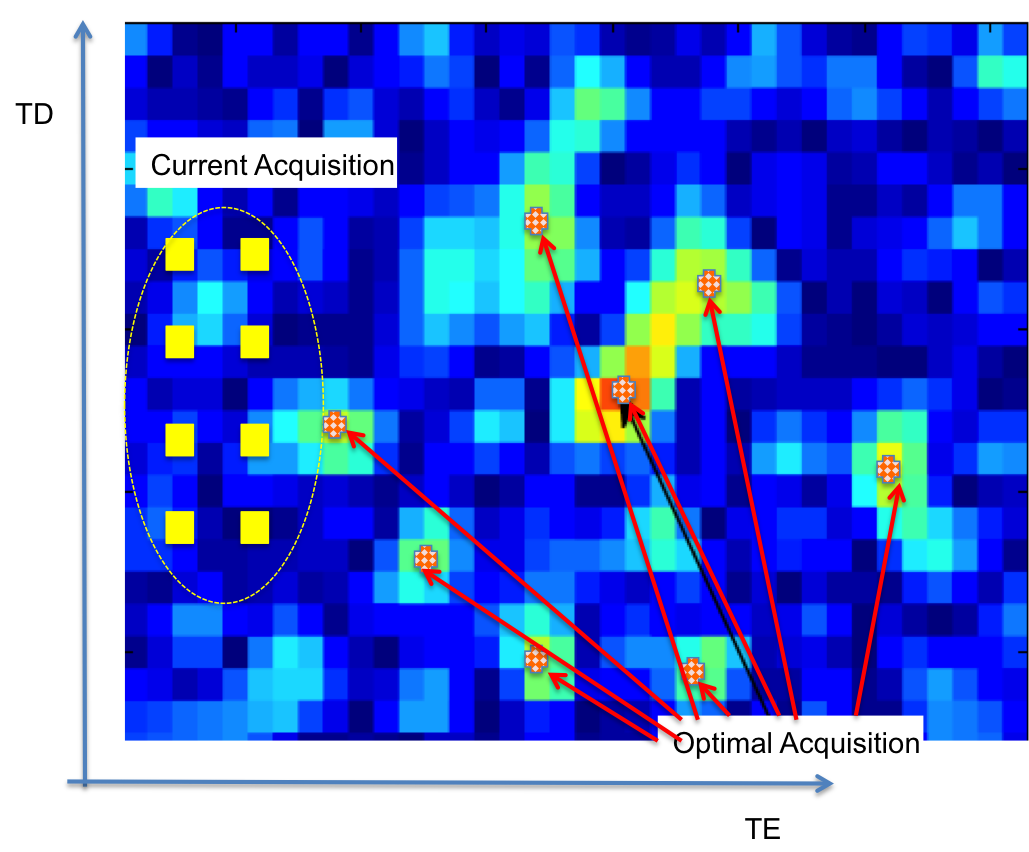
\includegraphics[width=.7\textwidth]{\picdir/MIMapTDTE.png} 
\caption{ 
Information content as function of $(T_D, T_E) \in \mathcal{F} = (0,4sec] \times (0,140ms] \subset \mathbb{R}^2 $.
The feasible set, $\mathcal{F} $, 
is determined by the pulse sequence acquisition physics.
}\label{fig:MIMapTDTE}
\end{figure}

%%%%%%%%%%%%%%%%%%%%%%%%%%%%%%%%%%%%%%%%%%%%%%%%%%%%%%%%%%%%%%%%
\section{Bayesian Learning}
%%%%%%%%%%%%%%%%%%%%%%%%%%%%%%%%%%%%%%%%%%%%%%%%%%%%%%%%%%%%%%%%

The `score' function from 
\cite{seeger2010optimization} is the mutual information between the desired measurement $\tilde{y}$
and the image $u$ conditioned on existing measurements $y$.
\[ 
\mathcal{S}   =  I(U;\tilde{Y}|Y) =  H(U|Y) - H(U|\tilde{Y},Y)   
\]
This has a very intuitive interpretation.  The current measure of uncertainty
in the parameter recovery (reconstruction) is $H(U|Y)$ for the given data, $Y$. 
The measure of uncertainty in the parameter recovery (reconstruction) for
 a new measurement, $\tilde{Y}$, is $H(U|Y,\tilde{Y})$.
The measurement, $\tilde{Y}$, is `optimal' when is reduction
in uncertainty in the parameter recovery (reconstruction) is maximized.

We will assume that the joint probability between (measurement, acquisition) pairs is  jointly normal.
The joint probability of signal measurements as a function of design parameters is assumed to be indepdent. 
% TODO work out
\[
 \begin{split}
   p(y_1,y_2|u,k_1,k_2)  & =
      C      \exp{
                \begin{bmatrix}
                 y_1 - \mu_1 \\
                 y_2 - \mu_2 \\
                \end{bmatrix}^\top
                \begin{bmatrix}
                 P^{-1}_{11} & 0      \\
                   0    & P^{-1}_{22} \\
                \end{bmatrix}
                \begin{bmatrix}
                 y_1 - \mu_1 \\
                 y_2 - \mu_2 \\
                \end{bmatrix}
                 }
    =  
      \underbrace{
         C_1    \exp{
                \|
                 y_1(u,k_1) - \mu_1
                \|_{P_{11}}
                  }}_{p(y_1|u,k_1)} 
      \underbrace{
         C_2    \exp{
                \|
                 y_2(u,k_2) - \mu_2
                \|_{P_{22}}
                  }}_{p(y_2|u,k_2)} 
 \end{split}
\]
For simplicity of notation, assume that two measures arise from two distinct acquisition parameters such that the dependence  on $k$ is assumed:
$
   p(y_1,y_2|u)  = p(y_1|u) p(y_2|u) 
$.
The joint distribution for the measurements is generally correlated through the model.
\[
   p(y_1,y_2)  = \int_U p(y_1,y_2,u) du = \int_U p(y_1,y_2|u)  p(u) du 
               = \int_U p(y_1|u) p(y_2|u) p(u) du 
  \qquad
 p(u|y_i) = \frac{ p(u,y_i)}{ p(y_i)}
        = \frac{ p(y_i|u) p(u)}{ p(y_i)}
\]
\[
   p(y_2|y_1)  = \frac{p(y_1,y_2)}{p(y_1)}
               = \frac{1}{p(y_1)}
                 \int_U p(y_1|u) p(y_2|u) p(u) du 
               = \int_U \frac{p(y_1|u)}{p(y_1)} p(y_2|u) p(u) du 
               = \int_U p(u|y_1) p(y_2|u)  du 
\]
\[
 p(y_i)  =  \int_U p(y_i|u)  p(u) du  
\]

Under these assumptions,
 the model for probability of parameters condition on the joint probability of
the data reduces to the probabulity of the parametery recovery (reconstruction) with respect
to the data multiplied by the probability of the new measurements given the 
parametery recovery (reconstruction) \cite{seeger2010optimization}. 
 \[
 p(u|\tilde{y},y) = \frac{ p(u,\tilde{y},y)}{ p(\tilde{y},y)}
                  = \frac{ p(\tilde{y},y|u) p(u) }{ p(\tilde{y},y)}
                  = \frac{ p(\tilde{y}|u) p(y|u) p(u) }{ p(\tilde{y},y)}
                  = \frac{ p(\tilde{y}|u) p(y|u) p(u) }{ p(\tilde{y},y)}
                  = p(\tilde{y}|u) p(u|y) \frac{ p(y) }{ p(\tilde{y},y)}
                  \propto p(u|y) p(\tilde{y}|u) 
\]
The final information gain may be computed as:
\[ 
\begin{split}
\mathcal{S}   =  I(U;\tilde{Y}|Y) &=  H(U|Y) - H(U|\tilde{Y},Y)   \\
            & = -\int_y \; dy \; p(y) \int_u \; du \;  p(u|y) \log p(u|y) 
              +  \int_{\tilde{y}}  \; d\tilde{y} \;\int_y  \; dy \; p(\tilde{y},y) \int_u  \; du \;p(u|\tilde{y},y) \log p(u|\tilde{y},y) \\
            & = -\int_y  \; dy \;p(y) \int_u  \; du \;p(u|y) \log p(u|y) 
              +  \int_{\tilde{y}}  \; d\tilde{y} \;\int_y  \; dy \; p(\tilde{y}|y) p(y)\int_u  \; du \;p(u|\tilde{y},y) \log p(u|\tilde{y},y) \\
            & =  \int_y  \; dy \;p(y)  \left(-\int_u  \; du \;p(u|y) \log p(u|y) 
              +  \int_{\tilde{y}}  \; d\tilde{y} \; p(\tilde{y}|y) \int_u  \; du \;p(u|\tilde{y},y) \log p(u|\tilde{y},y) \right) \\
\end{split}
\]
We have two options to compute the information gain $I(U;\tilde{Y}|Y)$  or scoring function $\mathcal{S}$ at this point:
\begin{enumerate}
  \item  Assume that the measurements are completely predicted by the model. ie
    \[
       p(y) =  \int_U p(y|u)  p(u) du  
    \]
  \item  Use Gaussian distribution around actual signal measurements $y^*$ and ignore the model predicted measurements
    \[
       p(y) =  \mathcal{N}(y^*,\sigma) = \exp\left(\frac{y - y^*}{\sigma} \right) \neq \int_U p(y|u)  p(u) du  
    \]
\end{enumerate}
{\color{red} @dmitchell412 how do we interpret this ? how does modeling errors affect this choice ? which is `better' ?
should we further separate into predicted measurement vs actual measurement ? ie Kalman Filter~\cite{maybeck1979stochastic}.
\[
  z = H y + \nu 
\qquad \Rightarrow \qquad
 I(U;\tilde{Y}|Z) 
\]
}


%%%%%%%%%%%%%%%%%%%%%%%%%%%%%%%%%%%%%%%%%%%%%%%%%%%%%%%%%%%%%%%%
\section{Overall Picture}
%%%%%%%%%%%%%%%%%%%%%%%%%%%%%%%%%%%%%%%%%%%%%%%%%%%%%%%%%%%%%%%%
The following diagram illustrates the general work-flow of the process:
\begin{figure}[h!!]
\center
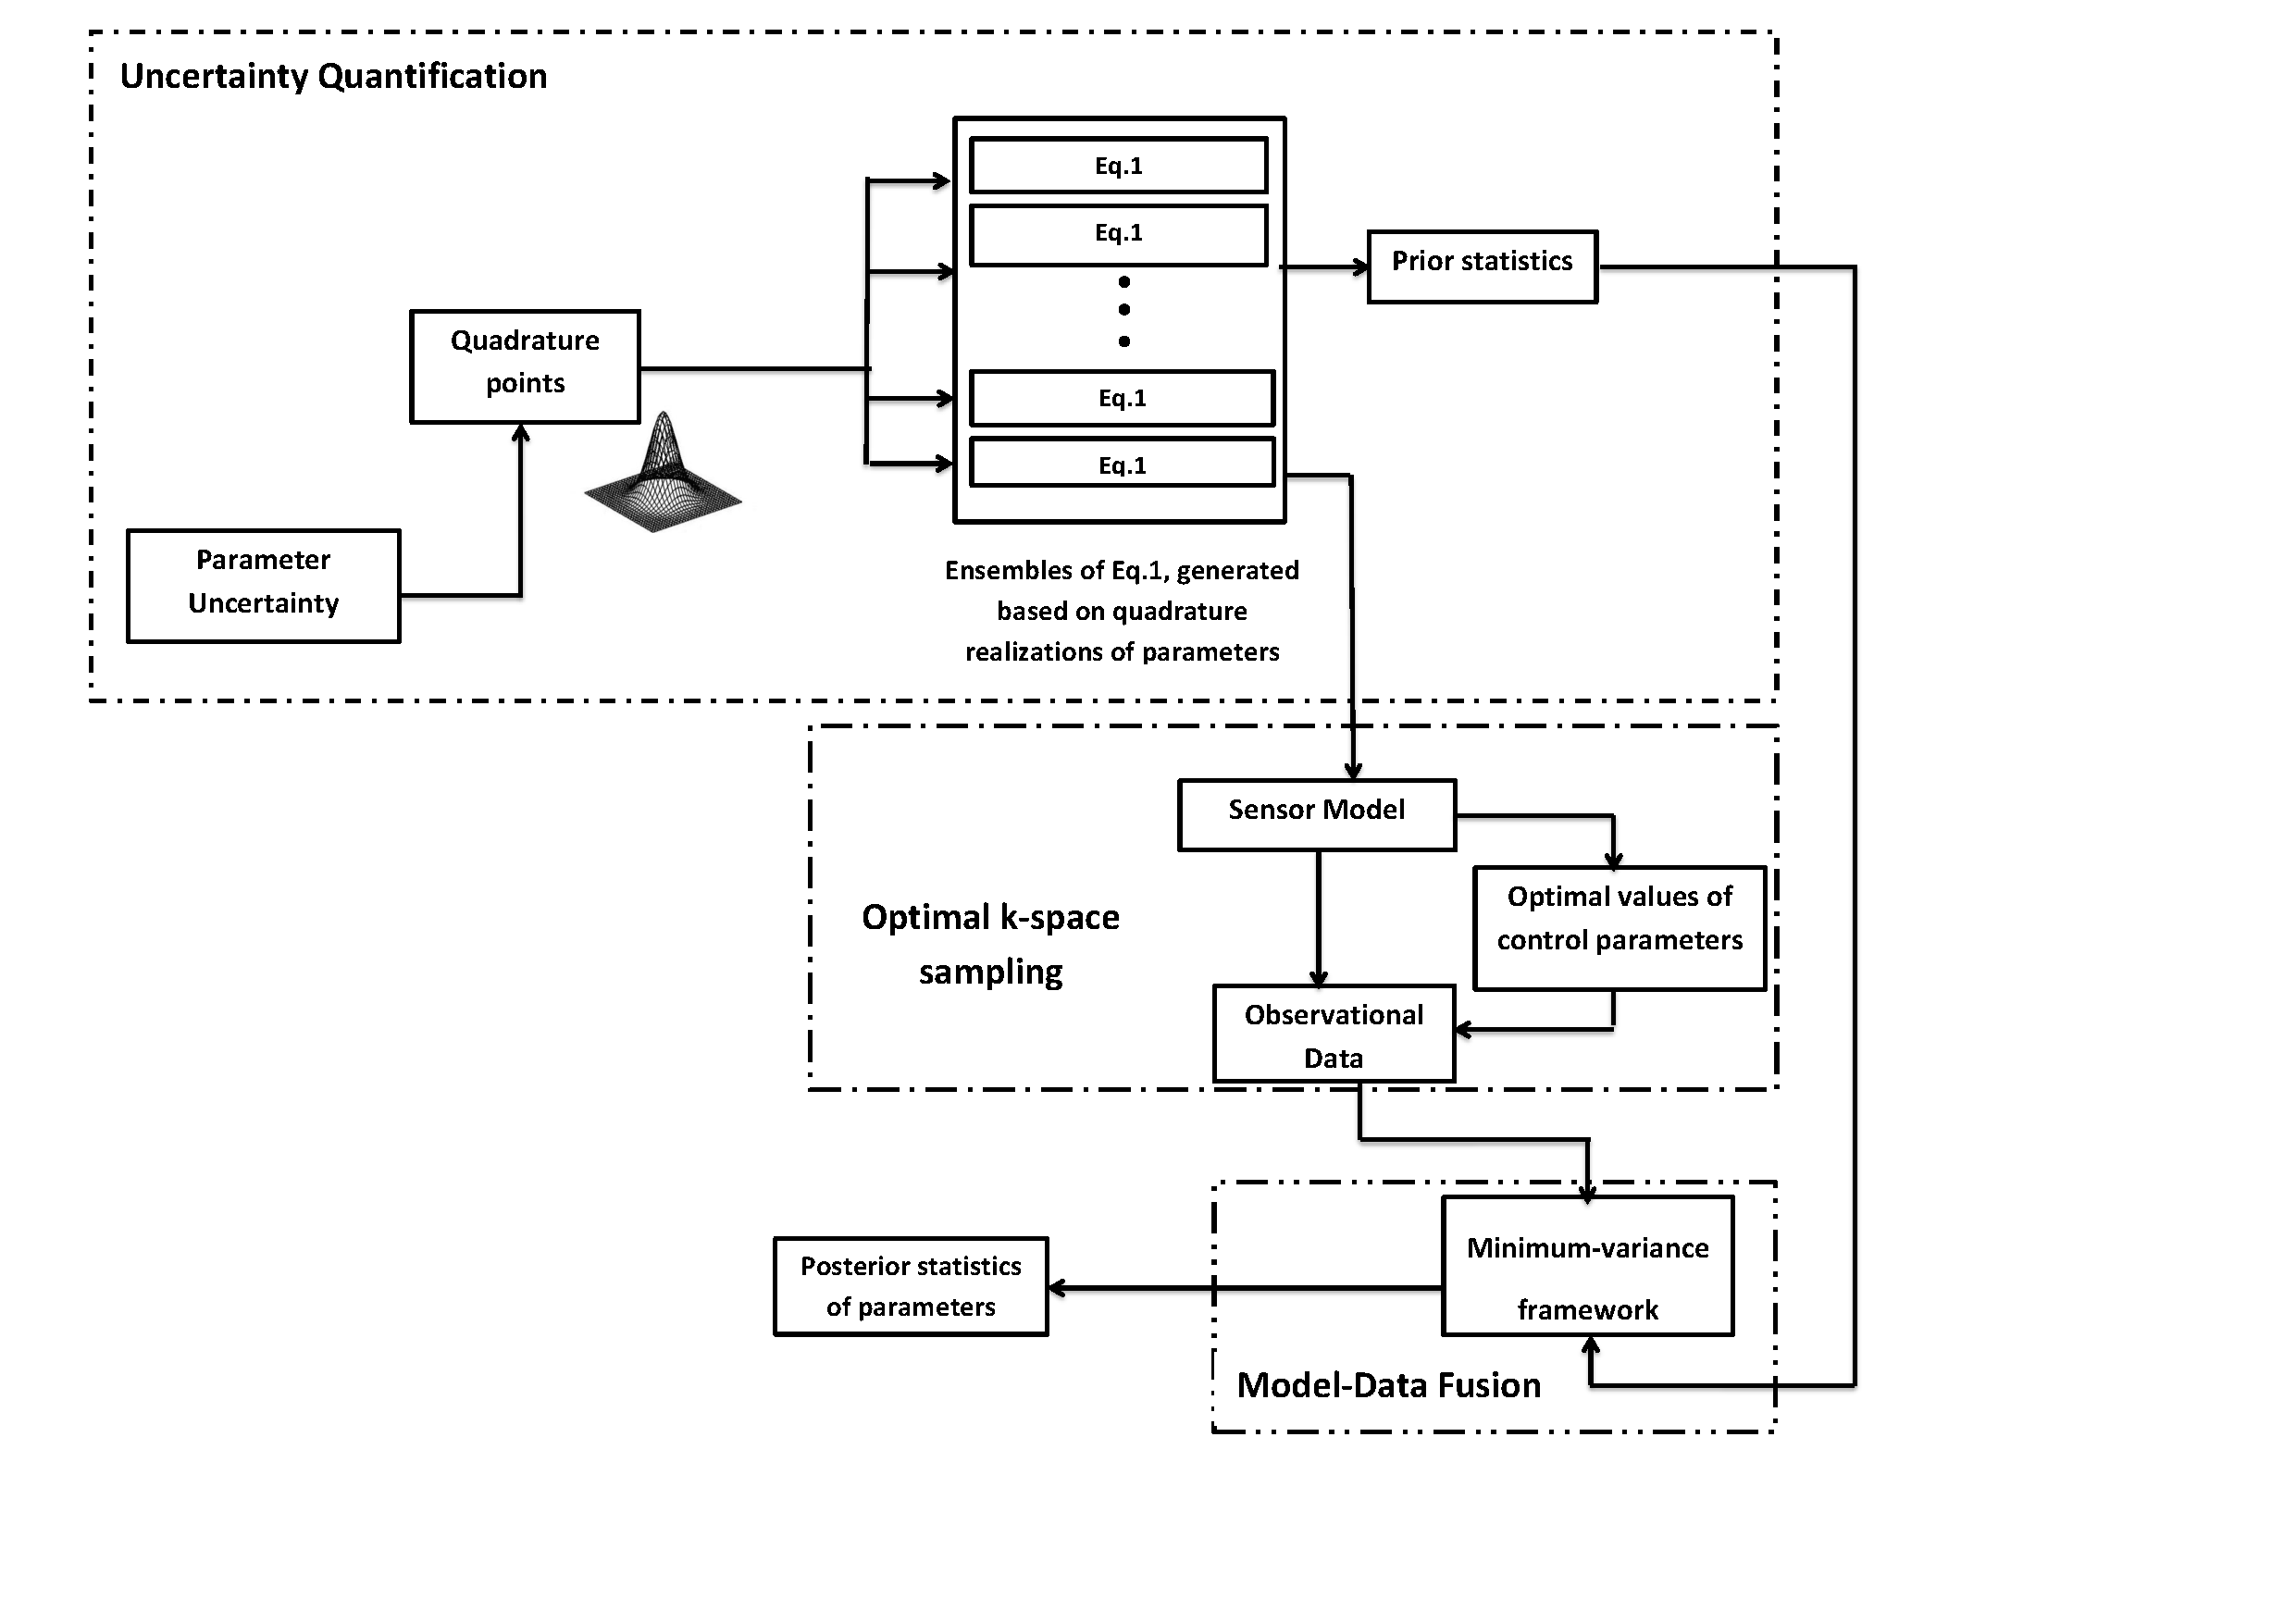
\includegraphics[trim = 1.5cm 3cm 8cm 0.5cm, clip,width=5in,height=4.5in]{\picdir/flowchart.pdf}
\caption{Schematic view of the estimation process}
\end{figure}

%%%%%%%%%%%%%%%%%%%%%%%%%%%%%%%%%%%%%%%%%%%%%%%%%%%%%%%%%%%%%%%%
\section{WIP - Inverse Problem Framework}\label{InverseProbFramework}
%%%%%%%%%%%%%%%%%%%%%%%%%%%%%%%%%%%%%%%%%%%%%%%%%%%%%%%%%%%%%%%%
\[
  \vec{z}  = \mathcal{G}(\theta) + \eta   \qquad   \eta \sim \mathcal{N}(0,\Sigma_z)
\]
\[
  p(z|\theta ) = \exp \left( \|\vec{z} -  \mathcal{G}(\theta)\|^2_{\Sigma_z} \right)
\]
\[
               d\left(\vec{z}, \mathcal{G}(\theta^*)\right) = 
   \min_{\theta \in \Omega} d\left(\vec{z}, \mathcal{G}(\theta)\right)
\qquad
\theta = \left(\mu_\text{CSF}, \mu_\text{GM}, \mu_\text{WM}, \mu_\text{Tumor} \right)
\]

%%%%%%%%%%%%%%%%%%%%%%%%%%%%%%%%%%%%%%%%%%%%%%%%%%%%%%%%%%%%%%%%
\section{WIP - T1, T2, M0 Reconstruction}
%%%%%%%%%%%%%%%%%%%%%%%%%%%%%%%%%%%%%%%%%%%%%%%%%%%%%%%%%%%%%%%%
\paragraph{Given}
the image space date for  multiple  acquistion parameters 
$\{ M_{TD}(\kk_1),M_{TD}(\kk_2), M_{TD}(\kk_2),... \}$,  \\
 $\kk_i=\{T_{R_i},T_{D_i},\theta_i,T_{E_i},\alpha_i\}$ 
{\color{red}(@kenphwang 2 delay times and 4 echoes correct?)},

The reconstruction algorithms for T1, T2, M0 is as follows:
\begin{itemize}
\item 
\item 
\item 
\end{itemize}

%%%%%%%%%%%%%%%%%%%%%%%%%%%%%%%%%%%%%%%%%%%%%%%%%%%%%%%%%%%%%%%%
%%%%%%%%%%%%%%%%%%%%%%%%%%%%%%%%%%%%%%%%%%%%%%%%%%%%%%%%%%%%%%%%
%%%%%%%%%%%%%%%%%%%%%%%%%%%%%%%%%%%%%%%%%%%%%%%%%%%%%%%%%%%%%%%%
%%%%%%%%%%%%%%%%%%%%%%%%%%%%%%%%%%%%%%%%%%%%%%%%%%%%%%%%%%%%%%%%
\nocite{*}
\bibliographystyle{apalike}
\bibliography{references}

\appendix
\section{Bayes - An intuitive example}\label{IntuitiveBayes}
Bayes theorem is fundamental to the approach and is immediately
follows from the definition of conditional probability
\[
\left.
\begin{split}
p(y|x)  \equiv  \frac{p(x,y)}{p(x)}  \\
p(x|y)  \equiv  \frac{p(x,y)}{p(y)} 
\end{split}
\right\}
\Rightarrow
p(y|x) p(x) = p(x,y) = p(x|y) p(y)
\Rightarrow
\hspace{-1in}
\begin{split}
p(y|x)  =\frac{ p(x|y) p(y) }{p(x) } \\
p(x|y)  =\frac{ p(y|x) p(x) }{p(y) } \\
\end{split}
\]

As a concrete example, consider the explicit two dimensional joint Gaussian
distribution as a medium for understanding. Here we have two random
variables $\mathbf{x}_1$ and $\mathbf{x}_2$ defined on the same probability
space, $\Omega$.
\[
\mathbf{x}_i: \Omega \rightarrow \mathbb{R}
\qquad
P\left( \left\{ \omega: 
\mathbf{x}_i (\omega) \in A
 \right\}\right)
=
\int_A p(\eta_i) d\eta_i
\]
Intuitively, if we are \textbf{given} the joint distribution,
$p(\eta_1,\eta_2)$, knowledge of the realization of one particular random
variable provides information on the realization of the second random
variable.
\[
      p(\eta_1,\eta_2)  = \frac{1}{2 \; \pi \; \sqrt{\det{\Sigma}}}
\exp\left( \frac{1}{2}
\begin{bmatrix}
\eta_1 - \mu_1 \\
\eta_2 - \mu_2 \\
\end{bmatrix}^\top
\underbrace{
\begin{bmatrix}
       \sigma_1^2        & r_{12} \sigma_1 \sigma_2 \\
r_{12} \sigma_1 \sigma_2 &          \sigma_2^2 \\
\end{bmatrix}
}_{\equiv \Sigma}
\begin{bmatrix}
\eta_1 - \mu_1 \\
\eta_2 - \mu_2 \\
\end{bmatrix}
\right)
\]

See \cite{maybeck1979stochastic} (Sec 3.10), characteristic functions 
are used to show that individual marginal
densities of joint  Gaussian random variable is also Gaussian.
\[
p(\eta_1) = 
\int_{\eta_2}
      p(\eta_1,\eta_2)
\;d\eta_2
 = \frac{1}{ \sqrt{2 \; \pi \; \sigma_2^2}} \exp\left( - \frac{(\eta_1 -
\mu_1)^2}{2 \sigma_1^2} \right)
\]

\[
p(\eta_2) = 
\int_{\eta_1}
      p(\eta_2,\eta_1)
\;d\eta_1
 = \frac{1}{ \sqrt{2 \; \pi \; \sigma_1^2}} \exp\left( - \frac{(\eta_2 -
\mu_2)^2}{2 \sigma_2^2} \right)
\]

Conditional probablity is \textit{defined} through the algegraic
reduction of the ratio of the joint and the marginal densities
\[
p(\eta_1|\eta_2) =  \frac{p(\eta_1,\eta_2)  }{p(\eta_2) }
 = \frac{1}{ \sqrt{2 \; \pi \; \sigma_{1|2}^2}}
    \exp\left( - \frac{(\eta_1 - \mu_{1|2})^2}{2 \sigma_{1|2}^2} \right)
 = 
\frac{p(\eta_1)}{p(\eta_2)}
   \frac{1}{ \sqrt{2 \; \pi \; \sigma_{2|1}^2}}
    \exp\left( - \frac{(\eta_2 - \mu_{2|1})^2}{2 \sigma_{2|1}^2} \right)
\]
\[
\mu_{1|2} =  \mu_1 - 
       \frac{r_{12} \sigma_1 \sigma_2 }{\sigma_2^2}
       (\eta_2 - \mu_2)
\qquad
\sigma_{1|2} = 
\sigma_1^2  - 
       \frac{(r_{12} \sigma_1 \sigma_2 )^2}{\sigma_2^2}
\]
\[
\mu_{2|1} =  \mu_2 - 
       \frac{r_{12} \sigma_1 \sigma_2 }{\sigma_1^2}
       (\eta_1 - \mu_1)
\qquad
\sigma_{2|1} = 
\sigma_2^2  - 
       \frac{(r_{12} \sigma_1 \sigma_2 )^2}{\sigma_1^2}
\]


%%%%%%%%%%%%%%%%%%%%%%%%%%%%%%%%%%%%%%%%%%%%%%%%%%%%%%%%%%%%%%%%
\section{Information theory identities}
%%%%%%%%%%%%%%%%%%%%%%%%%%%%%%%%%%%%%%%%%%%%%%%%%%%%%%%%%%%%%%%%


Key ideas of active Bayesian learning follows from the  definition of conditional 
mutual information~\cite{cover2012elements} and \textit{repeeated} application of
 the definition of conditional probability and conditional entropy.
\[
 p(x,y|z) \equiv \frac{p(x,y,z)}{p(z)} 
               = \frac{p(x|y,z)p(y,z)}{p(z)}
               =       p(x|y,z)p(y|z)
\]
\[
 H(Y|X  ) \equiv E_x \left[ H(Y|X=x) \right] =  \sum_x p(x) H(Y|X=x) =  -\sum_{x} p(x) \sum_{y} p(y|x) \log p(y|x) 
\]
\[ 
\begin{split}
I(X;Y|Z) &\equiv \sum_x \sum_y \sum_z p(x,y,z) \log  \frac{  p(x,y|z)       }{p(x|z)p(y|z)} 
             =   \sum_x \sum_y \sum_z p(x,y,z) \log  \frac{  p(x|y,z)p(y|z) }{p(x|z)p(y|z)} 
             =   \sum_x \sum_y \sum_z p(x,y,z) \log  \frac{  p(x|y,z)       }{p(x|z)      } \\
         &   =  -\sum_x \sum_y \sum_z p(x,y,z) \log                           p(x|z)       
             +   \sum_x \sum_y \sum_z p(x,y,z) \log          p(x|y,z)                       \\
         &   =  -\sum_x \sum_z        p(x,  z) \log                           p(x|z)       
             +   \sum_x \sum_y \sum_z p(x|y,z) p(y,z)  \log  p(x|y,z)                       \\
         &   =  -\sum_z p(z) \sum_x p(x|z) \log p(x|z) 
             +   \sum_y \sum_z  p(y,z) \sum_x p(x|y,z) \log p(x|y,z)                      
             =   H(X|Z) - H(X|Y,Z) 
\end{split}
\]

\end{document}
